\documentclass[compilation.tex]{subfiles}

\begin{document}

\section{1983 Soviet nuclear false alarm incident}

\subsection{Overview}

\begin{wrapfigure}[11]{r}[1em]{0.4\textwidth}
	\vspace{-\baselineskip}
	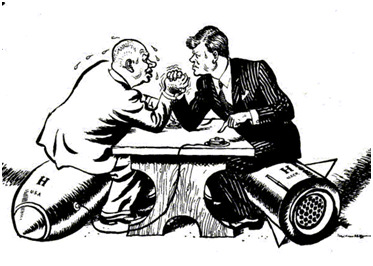
\includegraphics[scale=0.80]{fist-fight.png}
\end{wrapfigure}

The year is 1983, a time when the relations between the US and the Soviet Union were severely strained.

Four years before, the Soviet had deployed fourteen SS-20 / RSD-10 theatre nuclear missiles (1979) and consequent NATO response consisting in the deployment of 108 Pershing II missiles ready to target Western  Europe.

Since 1981, the United States had been running psychological operations against the Soviet Union to test their radars’ capabilities and to demonstrate the US’ power.
Clandestine naval operations near the Soviet territory and bomber flights to their border several times a week that turned away at the last moment are some of the examples of this type of aggression.

\subsection{The incident}

That’s why Stanislav Petrov, a lieutenant colonel in Soviet Air Defense Forces and the officer of the Serpukhov-15 bunker in charge of the Soviet early warning satellites code-named Oko had orders to, in the detection of incoming missiles, start an immediate and compulsory counterattack against the United States.

On 26 September, the bunker’s computers detected one intercontinental ballistic missile heading towards the USSR from the USA.
Petrov's responsibilities included observing the satellite early warning network and notifying his superiors of any impending nuclear missile attack against the Soviet Union.

\begin{wrapfigure}[12]{r}[1em]{0.38\textwidth}
	\vspace{-\baselineskip}
	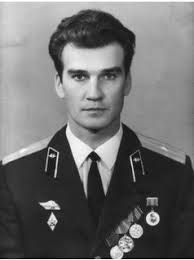
\includegraphics[scale=0.80]{stanislav-petrov.png}
\end{wrapfigure}

A suspicion was raised in the lieutenant’s mind that this occurrence must have been the result of a software malfunction (the system’s reliability had already been questioned in the past) since a first strike from the US was likely to involve hundreds of simultaneous missile launches in order to disable the Soviet Union’s means of counterattack, so he decided not to follow his obligations and not retaliate, avoiding World War III.
Later that day the computer detected four more incoming missiles that he dismissed as false alarms once again despite having no direct means to confirm this.

\begin{wrapfigure}[11]{r}[1em]{0.38\textwidth}
	\vspace{\baselineskip}
	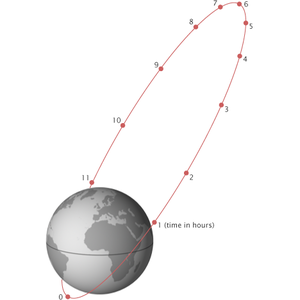
\includegraphics[scale=0.50]{earth-orbit.png}
\end{wrapfigure}

\subsubsection{The Bug and its solving}

It was subsequently determined that the false alarms were caused by a bug in the Soviet software that failed to filter out false missile detections caused by sunlight reflecting off cloud-tops, an error later corrected by cross-referencing a geostationary satellite.

\subsection{Aftermath}

Petrov first was praised for his actions and promised a reward, but later underwent intense questioning by the Soviets to justify his actions. 

In the end, he received no reward, probably (as Petrov speculates) because the officials and the scientists in charge of the system were embarrassed by the incident and other bugs later found and if he had been commended,  they would’ve had to be punished severely.
The story was buried having only surfaced in 1990 due to the publication of Votintsev’s memoirs.

Petrov was later commended and praised in the USA by several associations having won the Dresden Preis award in Germany, 2013.

\subsection{Lessons Learned}

When a piece of software is created, every possible case needs to be covered to avoid events like these.
Software is part of our lives and will be with the passing of time, even more.
Some say it will hold our lives in the future, in this case, I think it did because a lot of people could’ve died because of this problem and the world as we know it today, wouldn’t exist.
Everyone forgets something and there is no combination of tools to consider every possible case regarding a program, only the human mind, which we know can fail us sometimes and be the changing factor between a faulty code that can start a world war and a code that protects a country and its inhabitants from outside attacks.

\nocite{*}

\end{document}